%%%%%%%%%%%%%%%%%%%%%%%%%%%%%%%%%%%%%%%%%%%%%%%%%%%%%%%%%%%%%%%%%%%%%%%%%%%%%%%%%%%%%
\section{Introduction}\label{sec:mtd_intro}
%%%%%%%%%%%%%%%%%%%%%%%%%%%%%%%%%%%%%%%%%%%%%%%%%%%%%%%%%%%%%%%%%%%%%%%%%%%%%%%%%%%%%

HAWC's current software suite, plugins to 3ML, does not fully utilize computational advancements of recent decades.
Said advancements include the proliferation of Graphical Processing Units (GPUs), and multithreading on multi-core processors.
The analysis described in \Cref{sec:glory_duck} took up to 3 months of human time waiting for the full gambit of data analysis and simulation of background to run.
Additionaly, with the addition of a 2D binning scheme, $f_\mathrm{hit}$ and NN, the expected compute time is expected to grow further.
Although excessive computing time was, in part, from an intense use of a shared computing cluster, it was evident that there was room for improvement.
In HAWC's next generation dSph DM search, I decided to develop codes that would utilize the multi-core processors on modern high performance computing clusters.
The results of this work are featured in this chapter and brought a human timing improvement to computation that scales as $1/N$ where $N$ is the number of threads.

%%%%%%%%%%%%%%%%%%%%%%%%%%%%%%%%%%%%%%%%%%%%%%%%%%%%%%%%%%%%%%%%%%%%%%%%%%%%%%%%%%%%%
\section{Dataset and Background}\label{sec:mtd_databgd}
%%%%%%%%%%%%%%%%%%%%%%%%%%%%%%%%%%%%%%%%%%%%%%%%%%%%%%%%%%%%%%%%%%%%%%%%%%%%%%%%%%%%%

This section enumerates the data and background methods used for HAWC's multi-threaded study of dSphs.
\Cref{sec:mtd_data} and \Cref{sec:mtd_tools} are most useful for fellow HAWC collaborators looking to replicate a multithreaded dSph DM search.

%%%%%%%%%%%%%%%%%%%%%%%%%%%%%%%%%%%%%%%%%%%%%%%
\subsection{Itemized HAWC files}\label{sec:mtd_data}
%%%%%%%%%%%%%%%%%%%%%%%%%%%%%%%%%%%%%%%%%%%%%%%

\begin{itemize}
    \item Detector Resolution: \texttt{refit-Pass5-Final-NN-detRes-zenith-dependent.root}
    \item Data Map: \texttt{Pass5-Final-NN-maptree-ch103-ch1349-zenith-dependent.root}
    \item Spectral Dictionary: \texttt{HDMSpectra\_dict\_gamma.npy}
\end{itemize}

% %%%%%%%%%%%%%%%%%%%%%%%%%%%%%%%%%%%%%%%%%%%%%%%
\subsection{Software Tools and Development}\label{sec:mtd_tools}
%%%%%%%%%%%%%%%%%%%%%%%%%%%%%%%%%%%%%%%%%%%%%%%

This analysis was performed using HAL and 3ML \cite{Abeysekara_2017, vianello2015multimission} in Python version 3.
I built software in collaboration with Michael Martin and Letrell Harris to implement the \emph{Dark Matter Spectra from the Electroweak to the Planck Scale} (HDM) \cite{HDMSpectra} and dSphs spatial model from \cite{DM_Strigari20} for HAWC analysis.
A NumPy dictionary of HDM was made for Py3.
The corresponding Python3 file is \texttt{HDMSpectra\_dict\_gamma.npy}.
These files can also be used for decay channels and tools are provided in HDM's \href{https://github.com/nickrodd/HDMSpectra/tree/master}{git repository} \cite{HDMSpectra}.
The analysis was performed using the Neural Network energy estimator for Pass 5.F.
A description of this estimator was provided in \Cref{sec:hawc}.\todo{define a subsection when it's written}
All other software used for data analysis, DM profile generation, and job submission to SLURM are also kept in my sandbox in the \href{https://gitlab.com/hawc-observatory/sandboxes/salaza82/dark_matter_hawc}{Dark Matter HAWC} project.
The above repository also incorporates the model inputs used previously in Glory Duck, described in \Cref{sec:glory_duck}

%%%%%%%%%%%%%%%%%%%%%%%%%%%%%%%%%%%%%%%%%%%%%%%
\subsection{Data Set and Background Description} \label{sec:mtd_data_bkgd}
%%%%%%%%%%%%%%%%%%%%%%%%%%%%%%%%%%%%%%%%%%%%%%%

The HAWC data maps used for this analysis contain 2565 days of data between runs 2104 (\todo{Day start}) and 7476 (\todo{day end}).
They were generated from pass 4.0 reconstruction.
The analysis is performed using the NN energy estimator with bin list:

\begin{itemize}
    \item[] \texttt{B1C0Ea}, \texttt{B1C0Eb}, \texttt{B1C0Ec}, \texttt{B1C0Ed}, \texttt{B1C0Ee}, \texttt{B2C0Ea}, \texttt{B2C0Eb}, \texttt{B2C0Ec}, \texttt{B2C0Ed}, \texttt{B2C0Ee}, \texttt{B3C0Ea}, \texttt{B3C0Eb}, \texttt{B3C0Ec}, \texttt{B3C0Ed}, \texttt{B3C0Ee}, \texttt{B3C0Ef}, \texttt{B4C0Eb}, \texttt{B4C0Ec}, \texttt{B4C0Ed}, \texttt{B4C0Ee}, \texttt{B4C0Ef}, \texttt{B5C0Ec}, \texttt{B5C0Ed}, \texttt{B5C0Ee}, \texttt{B5C0Ef}, \texttt{B5C0Eg}, \texttt{B6C0Ed}, \texttt{B6C0Ee}, \texttt{B6C0Ef}, \texttt{B6C0Eg}, \texttt{B6C0Eh}, \texttt{B7C0Ee}, \texttt{B7C0Ef}, \texttt{B7C0Eg}, \texttt{B7C0Eh}, \texttt{B7C0Ei}, \texttt{B8C0Ee}, \texttt{B8C0Ef}, \texttt{B8C0Eg}, \texttt{B8C0Eh}, \texttt{B8C0Ei}, \texttt{B8C0Ej}, \texttt{B9C0Ef}, \texttt{B9C0Eg}, \texttt{B9C0Eh}, \texttt{B9C0Ei}, \texttt{B9C0Ej}, \texttt{B10C0Eg}, \texttt{B10C0Eh}, \texttt{B10C0Ei}, \texttt{B10C0Ej}, \texttt{B10C0Ek}, \texttt{B10C0El}
\end{itemize}
Bin 0 was excluded as it has substantial hadronic contamination and poor angular resolution.

Background considerations and source selection was identical to \Cref{sec:gd_databgd}, and no additional arguements are provided here.
Many of the HAWC systematics explored in \Cref{sec:hawc_systematic} also apply for this DM search and are not added upon here.

%%%%%%%%%%%%%%%%%%%%%%%%%%%%%%%%%%%%%%%%%%%%%%%%%%%%%%%%%%%%%%%%%%%%%%%%%%%%%%%%%%%%%
\section{Analysis}\label{sec:mtd_analysis}
%%%%%%%%%%%%%%%%%%%%%%%%%%%%%%%%%%%%%%%%%%%%%%%%%%%%%%%%%%%%%%%%%%%%%%%%%%%%%%%%%%%%%

The analysis and its systematics are almost identical to \Cref{sec:gd_analysis}.
Importantly, we use the same \Cref{eq:id_dm_flux} and \Cref{eq:jfactor} for estimating the gamma-ray flux at HAWC from our sources.
We add on to the previous study with a search for DM decay.
The flux equations for DM decay are
\iddmdecay[\gamma]

with a new quantity, the \D factor, defined as
\dfactor
Software was written to accomodate DM decay from dSphs, however decay profiles were not received from \LS by the time of writing this tehsis.

%%%%%%%%%%%%%%%%%%%%%%%%%%%%%%%%%%%%%%%%%%%%%%%%%%
\subsection{$\frac{dN_\gamma}{dE_\gamma}$ - Particle Physics Component}\label{sec:mtd_particlephysics}
%%%%%%%%%%%%%%%%%%%%%%%%%%%%%%%%%%%%%%%%%%%%%%%%%%

For these spectra, we import HDM with Electroweak (EW) corrections and additional corrections for neutrinos above the EW scale \cite{HDMSpectra}.
The spectrum is implemented as a model script in astromodels for 3ML.
A comprehensive description of EW corrections and neutrino considerations are provided later in \todo{refeance MM nu duck}.

\begin{figure}[t]
    \centering{
        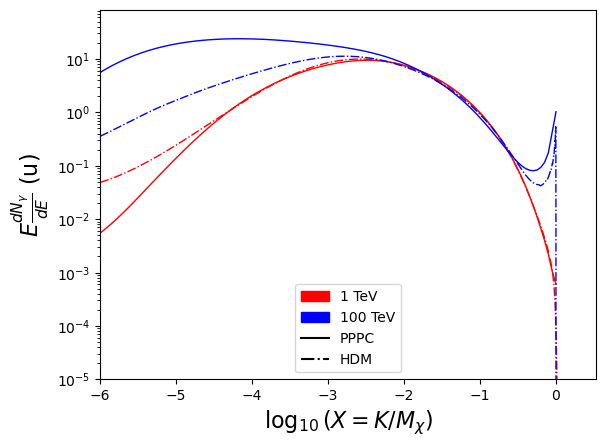
\includegraphics[scale=0.8]{figures/mtd_hawc_dm/pppc_vs_hdm.png}
    }
    \caption{Difference between spectral hypotheses from PPPC \cite{Cirelli_2011} and HDM \cite{HDMSpectra}. Shown is the expected DM annihilation spectrum for $\chi\chi \rightarrow W^-W^+$. Solid lines are spectral models with EW corrections from the PPPC. Dash-dot lines are spectral models from HDM. Red lines are models for $M_\chi = 1$ TeV. Blue lines represent models for $M_\chi = 100$ TeV.}
    \label{fig:pppc_vs_hdm}
\end{figure}

\Cref{fig:pppc_vs_hdm} demonstrates the impact of changes from HDM on DM
annihilation to W bosons.
A class in astromodels was developed to include HDM and is aptly named \texttt{HDMSpectra} within \texttt{DM\_models.py}.
The SM DM annihilation channels studied here are $\chi\chi \rightarrow$:
\begin{itemize}
    \item[] $e^+e^-$, $\mu^+\mu^-$, $\tau^+\tau^-$,$b\bar{b}$, $t\bar{t}$, $gg$, $W^+W^-$, $ZZ$, $c\bar{c}$, $u\bar{u}$, $d\bar{d}$, $s\bar{s}$, $\nu_e \overline{\nu_e}$, $\nu_\mu \overline{\nu_\mu}$, $\nu_\tau \overline{\nu_\tau}$, $\gamma\gamma$, $hh$.
\end{itemize}
For $\gamma\gamma$ and $ZZ$, a substantial fraction of the signal photons are expected to have total energy equal $m_\chi$ \cite{HDMSpectra}.
This introduces a $\delta$-function that is much narrower than the energy resolution of the HAWC detector.
To ensure that this feature is not lost in the likelihood fits, the 'line' feature is convolved with a gausian kernel with a $1\sigma$ width of $0.05 \cdot m_\chi$ and total kernel window of $\pm4\sigma$.
This difers from HAWC's previous line study where 30\% of HAWC's energy resolution was used for the kernel \cite{HAWC_dm_gammalines}.
The NN energy estimator's strength compared to $f_\mathrm{hit}$ at low gamma-ray energy enables smaller resolutions in addition to low energy tails in the spectral models \cite{HDMSpectra}.
$\chi\chi \rightarrow \gamma\gamma$ and $ZZ$ spectral hypotheses are shown in \Cref{fig:hdm_gamma_lines}.
Spectral models for the remaining annihilation channels are plotted for each $m_\chi$ in \Cref{fig:apdx_mtd_spectra}.

\begin{figure}[t]
    \centering{
    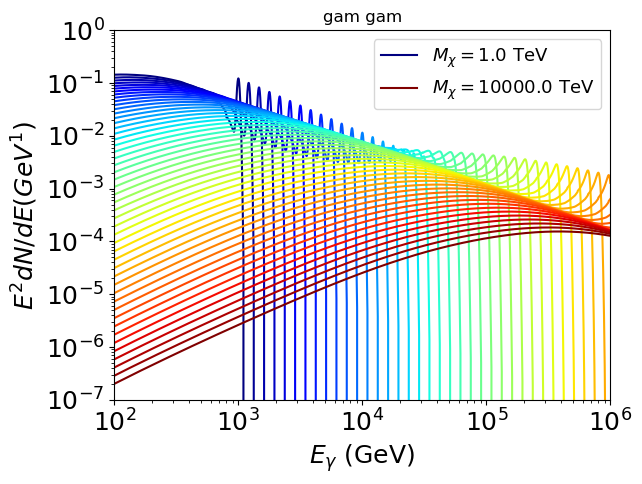
\includegraphics[scale=0.5]{figures/mtd_hawc_dm/hdm_gammagamma.png}
    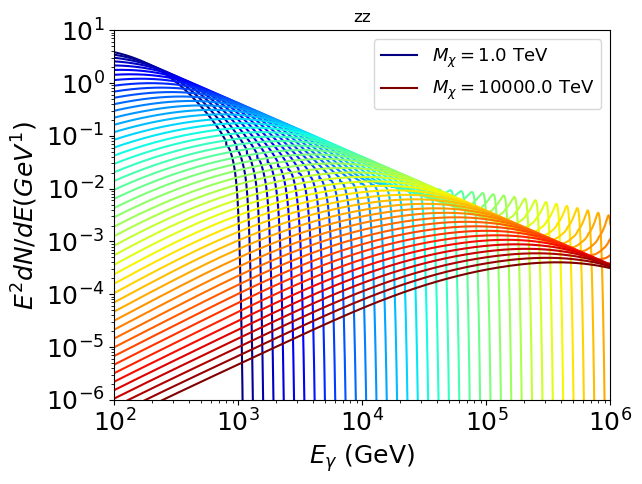
\includegraphics[scale=0.5]{figures/mtd_hawc_dm/hdm_zz.png}
    }
    \caption{Photon spectra for $\chi\chi \rightarrow \gamma\gamma$ (left) and $\chi\chi \rightarrow ZZ$ (right) after gaussian convolution of line features. Both spectra have $\delta$-features at photon energies equal to the DM mass. Bluer lines are annihilation spectra with lower DM mass. Redder lines are spectra from larger DM mass. All Spectral models are sourced from the Heavy Dark Matter models \cite{HDMSpectra}.}
    \label{fig:hdm_gamma_lines}
\end{figure}

%%%%%%%%%%%%%%%%%%%%%%%%%%%%%%%%%%%%%%%%%%%%%%%%%%
\subsection{\J and \D - Astrophysical Components}\label{sec:mtd_spatialmodel}
%%%%%%%%%%%%%%%%%%%%%%%%%%%%%%%%%%%%%%%%%%%%%%%%%%

The J-factor profiles for each source are imported from Louis Strigari et al. (referred to with \LS) \cite{DM_Strigari20}.
Profiles in $\frac{d\J}{d\Omega} (\theta)$ and $\frac{d\D}{d\Omega} (\theta)$ up to $\theta = 0.5^{\circ}$ were provided directly from the authors.
Map generation from these profiles were almost identical to \Cref{sec:gd_spatialmodel} except that a higher order trapezoidal integral was used for the normalization of the square, uniformly-spaced map:
\TrapIntegral
$\mathcal{K}$ is either \J or \D for the spatial distributions of annihilation or decay respectively.
$p$ is the angular side of one pixel in the map.
$w_{i,j}$ is a weight assigned the following ways:
\begin{itemize}
    \item[] $w_{i,j} = 1$ if $(\theta_{i,j}, \phi_{i,j})$ is fully within the region of integration
    \item[] $w_{i,j} = 1/2$ if $(\theta_{i,j}, \phi_{i,j})$ is on an edge of the region of integration
    \item[] $w_{i,j} = 1/4$ if $(\theta_{i,j}, \phi_{i,j})$ is on a corner of the region of integration
\end{itemize}
\Cref{fig:ls20_jfac_maps} shows the median and $\pm1\sigma$ maps used as input for DM annihilation studied by \LS.

\begin{figure}[t]
    \centering{
    \begin{tabular}{cccc}
        Source & $-1 \sigma$ & Median & $+1 \sigma$ \\
        \rotatebox[origin=c]{90}{Coma Berenices} &
        \raisebox{-.5\height}{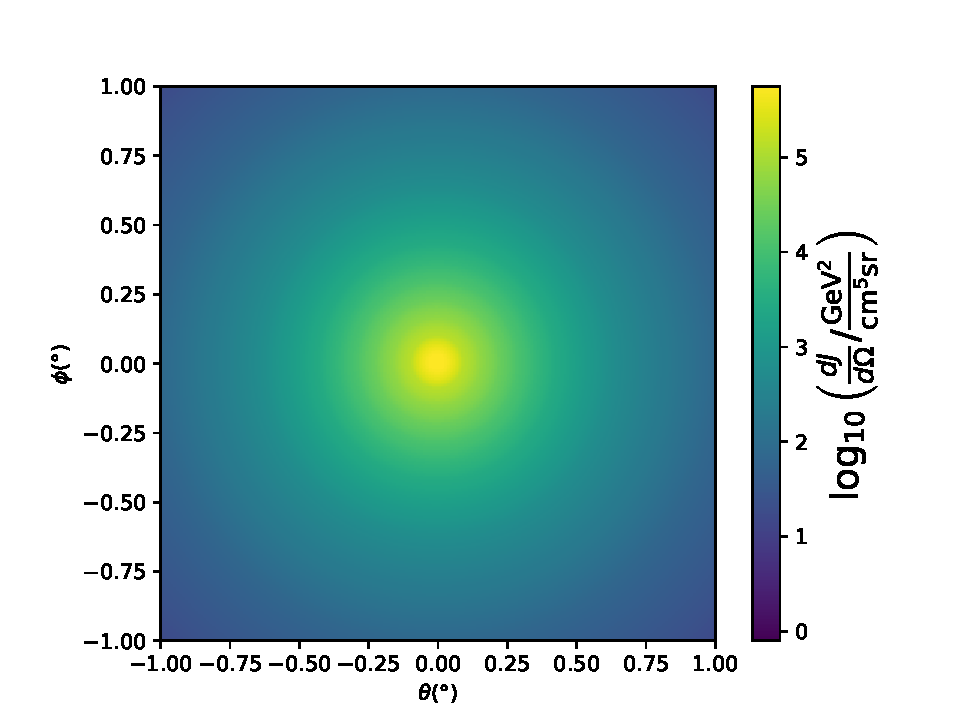
\includegraphics[scale=0.275]{figures/mtd_hawc_dm/ComaBerenices_Jm1_plot.pdf}} &
        \raisebox{-.5\height}{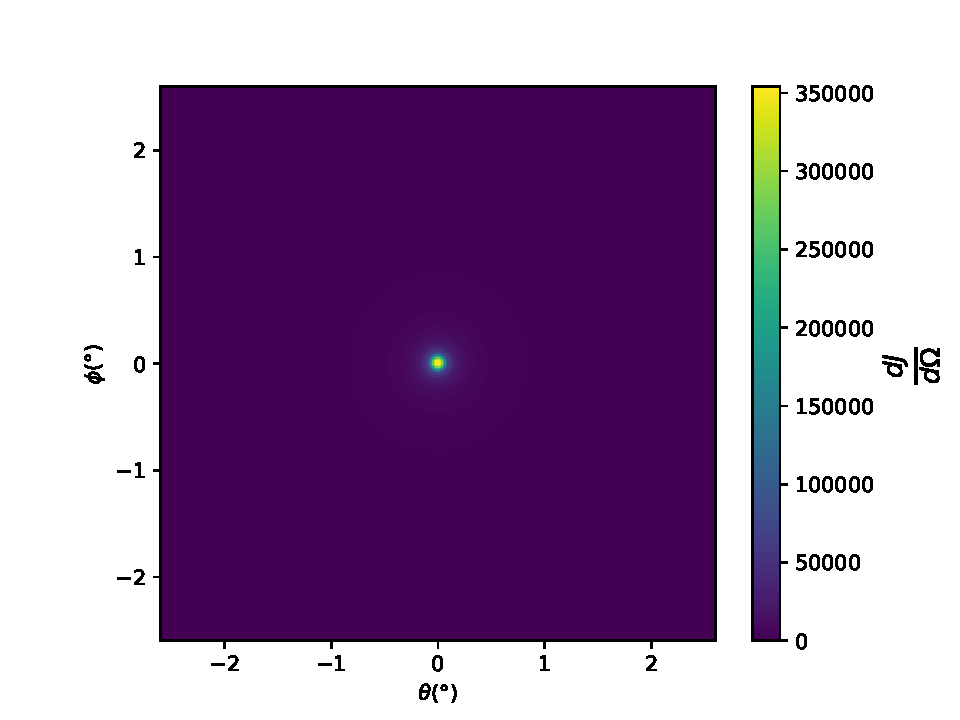
\includegraphics[scale=0.275]{figures/mtd_hawc_dm/ComaBerenices_J_plot.pdf}} &
        \raisebox{-.5\height}{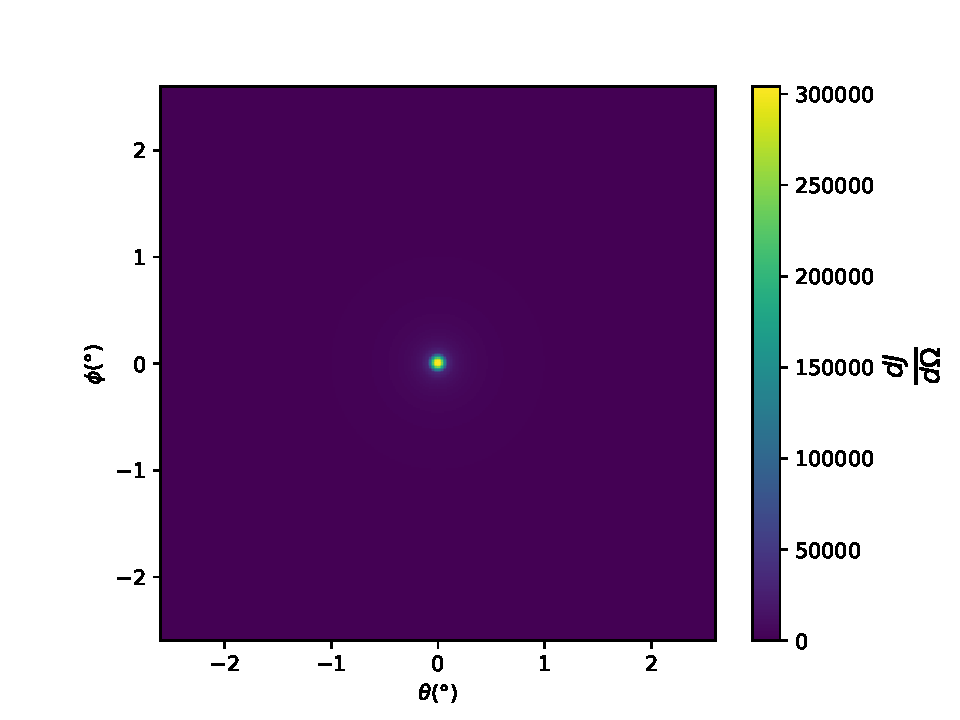
\includegraphics[scale=0.275]{figures/mtd_hawc_dm/ComaBerenices_Jp1_plot.pdf} }\\
        \rotatebox[origin=c]{90}{Draco} &
        \raisebox{-.5\height}{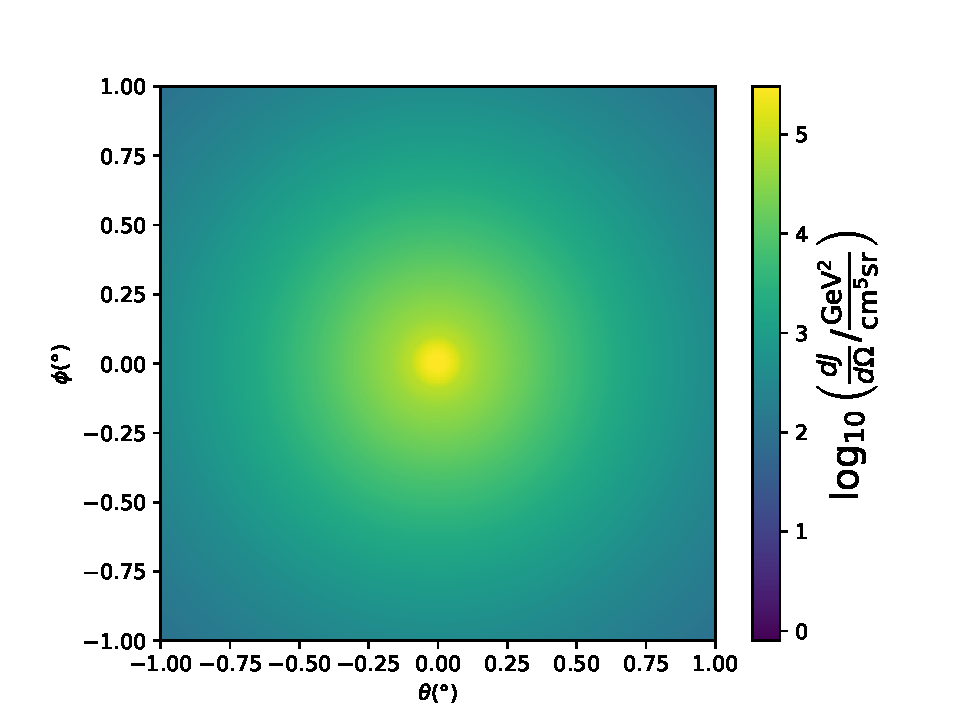
\includegraphics[scale=0.275]{figures/mtd_hawc_dm/Draco_Jm1_plot.pdf}} &
        \raisebox{-.5\height}{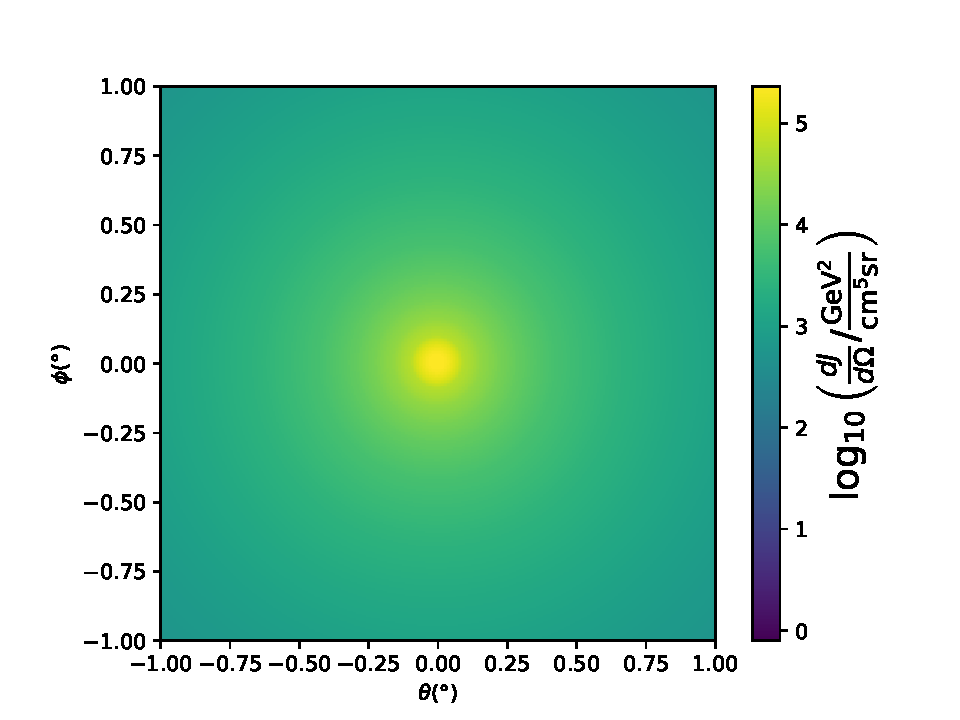
\includegraphics[scale=0.275]{figures/mtd_hawc_dm/Draco_J_plot.pdf}} &
        \raisebox{-.5\height}{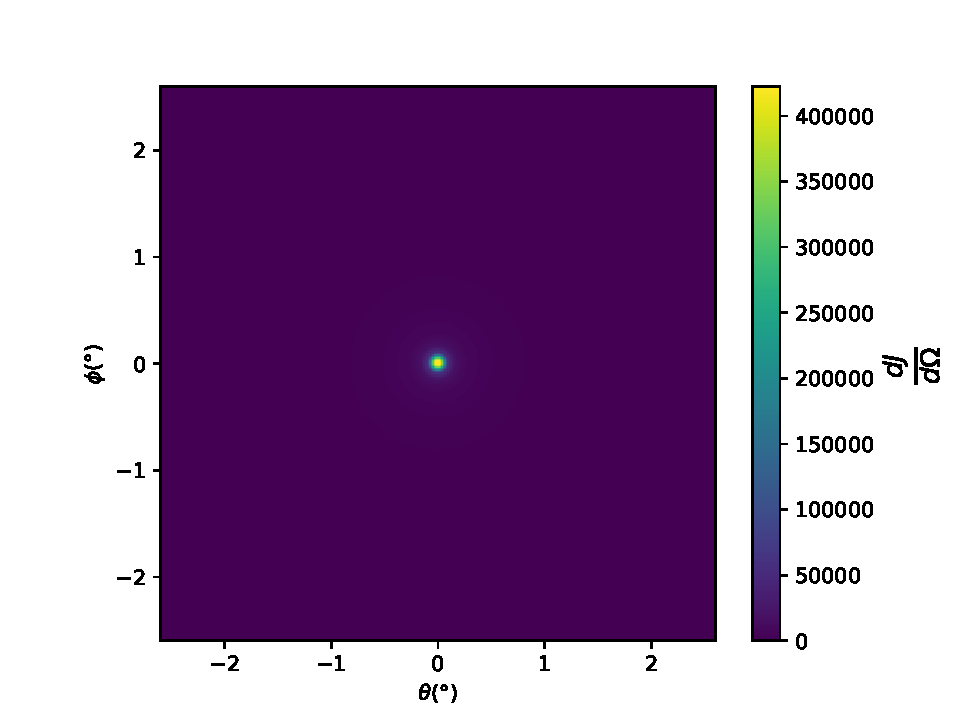
\includegraphics[scale=0.275]{figures/mtd_hawc_dm/Draco_Jp1_plot.pdf}} \\
        \rotatebox[origin=c]{90}{Segue1} &
        \raisebox{-.5\height}{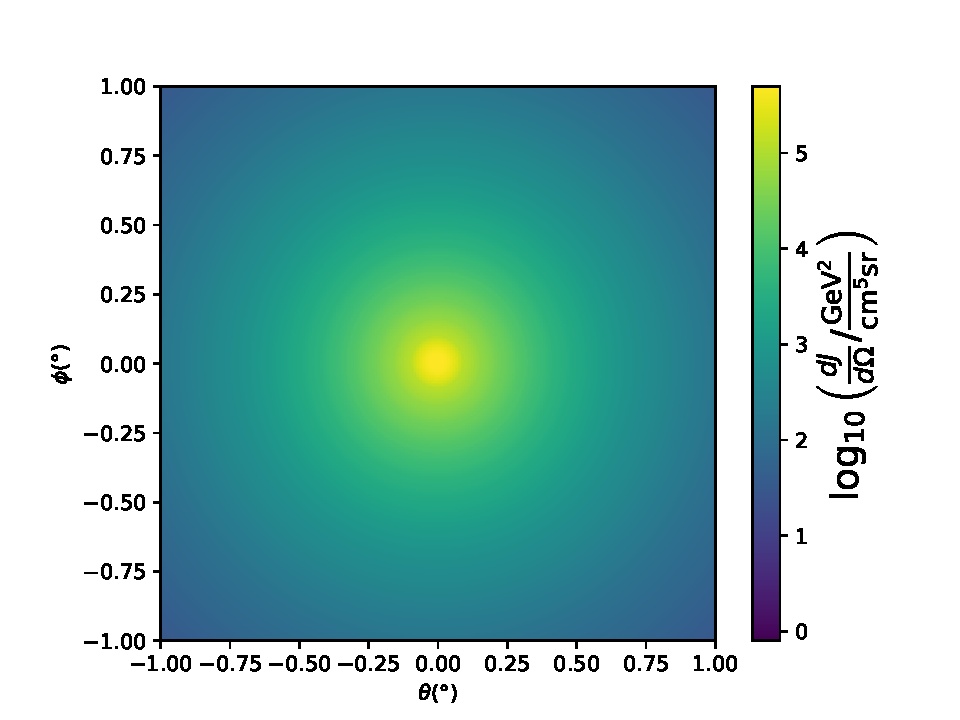
\includegraphics[scale=0.275]{figures/mtd_hawc_dm/Segue1_Jm1_plot.pdf}} &
        \raisebox{-.5\height}{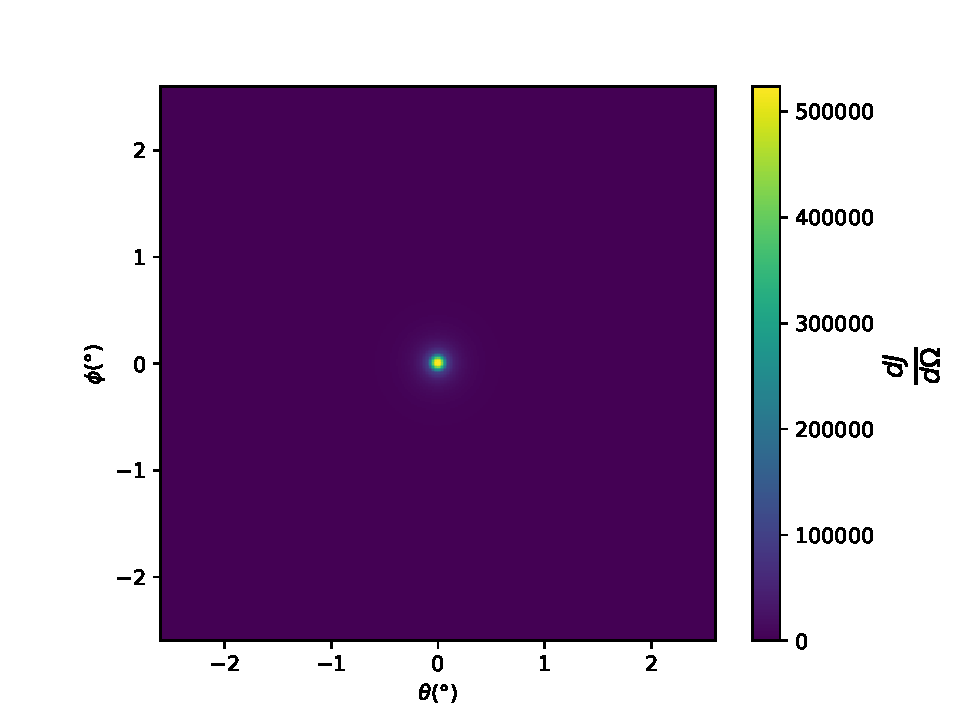
\includegraphics[scale=0.275]{figures/mtd_hawc_dm/Segue1_J_plot.pdf}} &
        \raisebox{-.5\height}{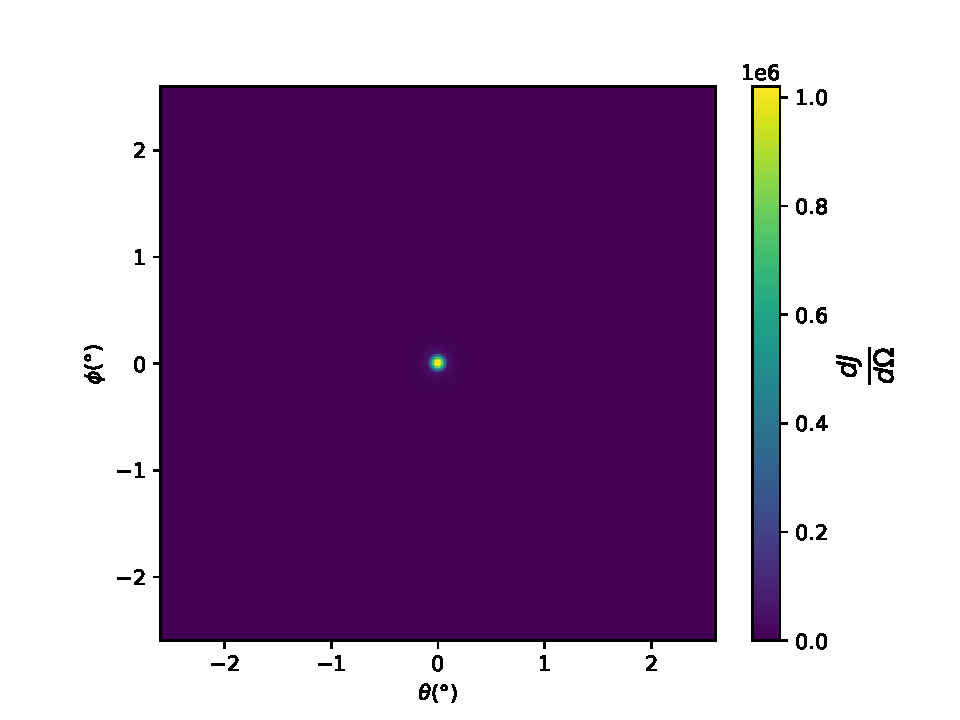
\includegraphics[scale=0.275]{figures/mtd_hawc_dm/Segue1_Jp1_plot.pdf}} \\
        \rotatebox[origin=c]{90}{Sextans} &
        \raisebox{-.5\height}{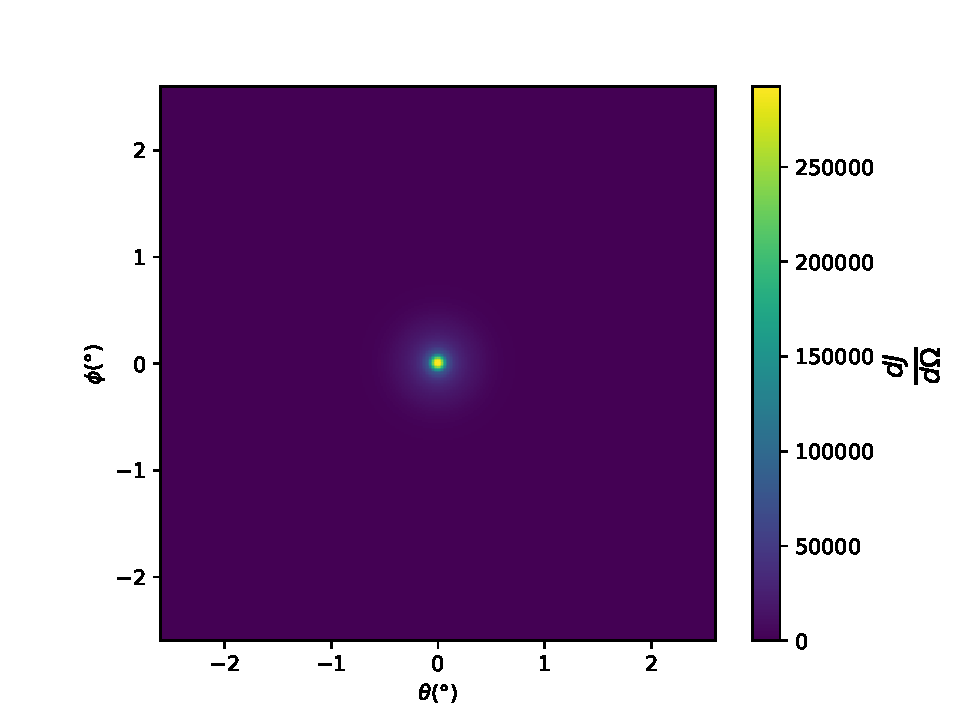
\includegraphics[scale=0.275]{figures/mtd_hawc_dm/Sextans_Jm1_plot.pdf}} &
        \raisebox{-.5\height}{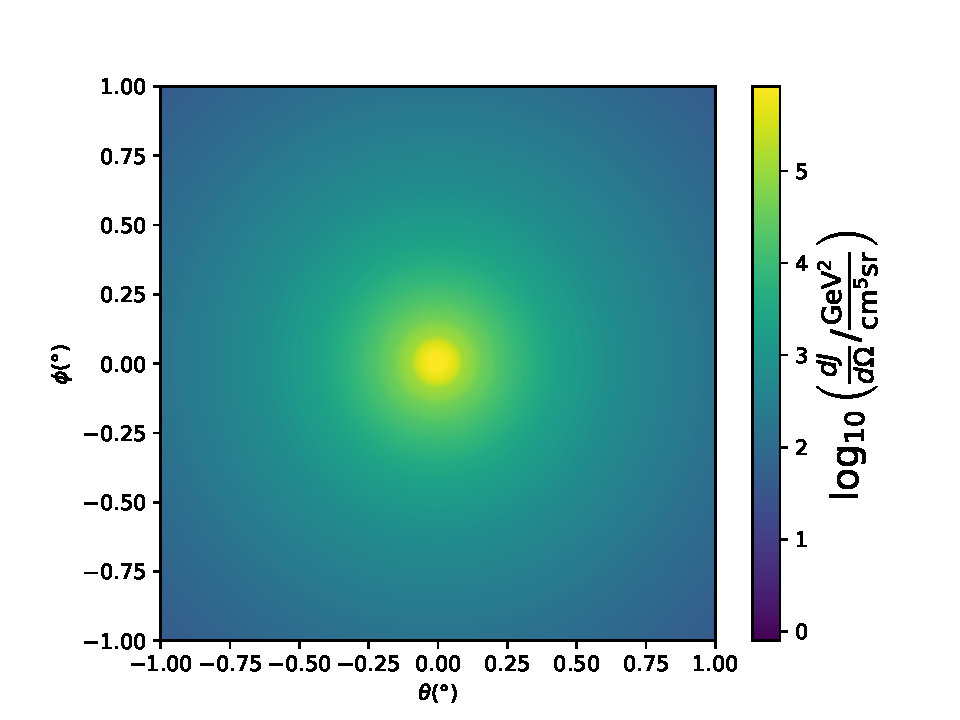
\includegraphics[scale=0.275]{figures/mtd_hawc_dm/Sextans_J_plot.pdf}} &
        \raisebox{-.5\height}{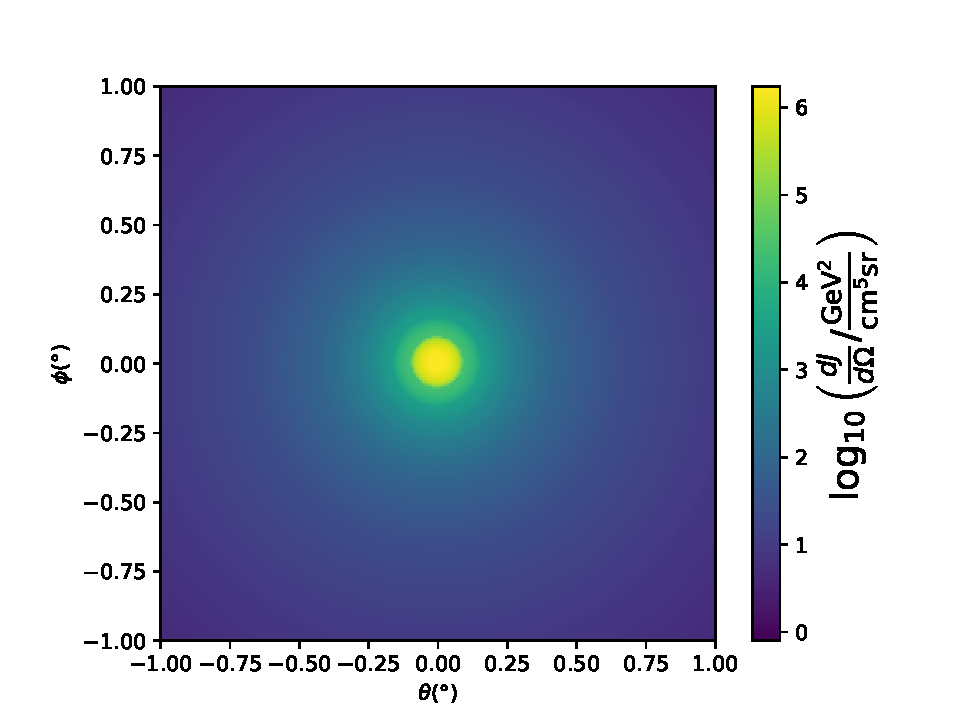
\includegraphics[scale=0.275]{figures/mtd_hawc_dm/Sextans_Jp1_plot.pdf}} \\
    \end{tabular}
    }
    \caption{$\frac{d\J}{d\Omega}$ maps for Coma Berenices, Draco, Segue1, and Sextans. Columns are divided for the $\pm1 \sigma$ uncertainties in $d\J/d\Omega$ around the median value from \LS \cite{DM_Strigari20}. Origin is centered on the specific dwarf spheroidal galaxies (dSph). $\theta$ and $\phi$ axes are the angular separation from the center of the dwarf. Axes are drawn roughly according to the energy sensitivity of HAWC.}
    \label{fig:ls20_jfac_maps}
\end{figure}

%%%%%%%%%%%%%%%%%%%%%%%%%%%%%%%%%%%%%%%%%%%%%%%%%%
\subsection{Source Selection and Annihilation Channels}\label{sec:mtd_srcs_y_chan}
%%%%%%%%%%%%%%%%%%%%%%%%%%%%%%%%%%%%%%%%%%%%%%%%%%

We use many of the dSphs presented in HAWC's previous dSph DM search \cite{Albert_2018}.
HAWC's sources for Glory Duck include Boötes I, Coma Berenices, Canes Venatici I + II, Draco, Hercules, Leo I, II, + IV, Segue 1, Sextans, and Ursa Major I + II.
A full description of all sources used in Glory Duck is found in \Cref{tab:gd_J_factor}.
Triangulum II was excluded from the Glory Duck analysis because of large uncertainties in its \J factor.
Ursa Minor was excluded from HAWC's contribution to the combination because the source extension model extended Ursa Minor beyond HAWC's field of view.
Ursa Minor was not expected to contribute significantly to the combined limit, so work was not invested in a solution to include Ursa Minor.

\begin{table}[b]
\centering
    \small{\begin{tabular}{cccc}
    \hline
    \hline
    \CellTopTwo{}
    Name & Distance & $l, b$ & $\log_{10}J$~(\LS set)\\
    & \scriptsize{(kpc)} &  \scriptsize{($\degree$)} & \scriptsize{$\log_{10}(\mathrm{GeV}^2 \mathrm{cm}^{-5}\mathrm{sr})$} \\
    \hline
    \CellTopTwo{}
    Coma Berenices & $44$ & $241.89,\: 83.61$ & $19.00^{+0.36}_{-0.35}$ \\
    \CellTopTwo{}
    Segue I & $23$ & $220.48,\: 50.43$ & $19.12^{+0.49}_{-0.58}$ \\
    \CellTopTwo{}
    Sextans & $86$ & $243.50,\: 42.27$ & $17.73^{+0.13}_{-0.12}$ \\
    \hline
    \hline
    \CellTopTwo{}
\end{tabular}}
    \caption{Summary of the relevant properties of the dSphs used in the present work. Column 1 lists the dSphs. Columns 2 and 3 present their heliocentric distance and galactic coordinates, respectively. Column 4 reports the \J-factors of each source given from the \LS studies and estimated $\pm 1\sigma$ uncertainties. The values $\log_{10}J$~(\LS set) \cite{DM_Strigari20} correspond to the mean \J-factor values  for a source extension truncated at $0.5^\circ$.}
    \label{tab:mtd_J_factor}
\end{table}

This analysis improves on the previous HAWC dSph paper \cite{Albert_2018} in the following ways.
Previously, the dSphs were treated and implemented as point sources.
For this analysis, dSphs are modeled and treated as extended source.
The impact of this change with respect to the upper limit is source dependent and is explored in \Cref{sec:gd_ext_limitvs_ptsrc}.
Previously, the particle physics model used for gamma-ray spectra from DM annihilation did not have EW corrections where the PPPC includes them.
Finally, the gamma-ray ray dataset is much larger.
The study performed here analyzes over 1000 days of data compared to 507.

The SM annihilation channels probed for the Glory Duck combination include $b\bar{b}$, $e\bar{e}$, $\mu\bar{\mu}$, $\tau\bar{\tau}$, $t\bar{t}$, $W^+W^-$, and $ZZ$.
A summary of all sources, with a description of each experiments' sensitivity to the source, is provided in \Cref{tab:gd_tabSummary}.
